\documentclass[12pt, a4paper]{article}

\nonstopmode
\usepackage{algorithm}
% \usepackage{algcompatible}
\usepackage{bm}
\usepackage{bbm}
\usepackage{algpseudocode}
\usepackage{amsmath} % flere matematikkommandoer
\usepackage{amssymb} % flere matematikkommandoer
\usepackage{arydshln}
\usepackage[utf8]{inputenc} % æøå
\usepackage[T1]{fontenc} % mere æøå
\usepackage{verbatim} % så man kan skrive ren tekst
\usepackage[all]{xy} % den sidste (avancerede) formel i dokumentet
\usepackage[margin=1in]{geometry}  % set the margins to 1in on all sides
\usepackage{graphicx}              % to include figures
\usepackage{amsfonts}              % for blackboard bold, etc
\usepackage{amsthm}                % better theorem environments
\usepackage{graphicx}
\usepackage{caption}
\usepackage{bm}
\usepackage{pgf}
\usepackage{fancyhdr}
\usepackage{hyperref}
\usepackage{stmaryrd}
\usepackage{mathtools}
\usepackage{multirow}
\usepackage{listings}
\usepackage{subcaption}
\usepackage[inline]{enumitem}
\usepackage[round]{natbib}
\usepackage{breqn}
\usepackage{tikz}
\usetikzlibrary{arrows,automata,fit,positioning, shapes, calc, fadings}

% various theorems, numbered by section

\newtheorem{thm}{Theorem}[section]
\newtheorem{lem}[thm]{Lemma}
\newtheorem{prop}[thm]{Proposition}
\newtheorem{cor}[thm]{Corollary}
\newtheorem{conj}[thm]{Conjecture}

\DeclareMathOperator{\id}{id}
\DeclareMathOperator*{\argmin}{argmin}
\DeclareMathOperator*{\argmax}{argmax}

\newcommand{\nn}{\mathcal{N}}
\newcommand{\uu}{\mathcal{U}}
\newcommand{\bb}{\mathcal{B}}
\newcommand{\ee}{\mathrm{e}}
\newcommand{\rd}[1]{\mathrm{#1}}
\newcommand{\bd}[1]{\mathbf{#1}}  % for bolding symbols
\newcommand{\RR}{\mathbb{R}}      % for Real numbers
\newcommand{\ZZ}{\mathbb{Z}}      % for Integers
\newcommand{\PP}{\mathbb{P}}      % for Prob
\newcommand{\EE}{\mathbb{E}}      % for Expectation
\newcommand{\II}{\mathbbm{1}}      % for Indicator fun
\newcommand{\NN}{\mathbb{N}}      % for Prob
\newcommand{\col}[1]{\left[\begin{matrix} #1 \end{matrix} \right]}
\newcommand{\eqsys}[2]{ \left[\!\!
    \begin{array}{#1} #2
    \end{array}
    \!\!\right]}
\newcommand{\comb}[2]{\binom{#1^2 + #2^2}{#1+#2}}
\newcommand{\sint}[1]{\shortintertext{#1}}
\newcommand{\CTL}[1]{\:\textrm{#1}\:}
\newcommand{\sat}{\:\:\textrm{\textbf{sat}}\:\:}
\newcommand{\pr}{\textrm{Pr}}
\newcommand{\grw}{m_{\mathcal{H}}}
\newcommand{\dvc}{d_{VC}}
\newtheorem{theorem}{Theorem}[section]
\newtheorem{lemma}{Lemma}[theorem]
\newtheorem{Lemma}{Lemma}[section]
\newtheorem{corollary}{Corollary}[theorem]
\newcommand{\lstbg}[3][0pt]{{\fboxsep#1\colorbox{#2}{\strut #3}}}
\newcommand{\kl}{\textrm{kl}}
\newcommand{\KL}{\textrm{KL}}
\newcommand{\hyp}{\mathcal{H}}
\lstdefinelanguage{diff}{
  basicstyle=\ttfamily\scriptsize,
  morecomment=[f][\lstbg{red!20}]-,
  morecomment=[f][\lstbg{green!20}]+,
  morecomment=[f][\textit]{@@},
  %morecomment=[f][\textit]{---},
  %morecomment=[f][\textit]{+++},
}

\newenvironment{gamedef}
{%
 \par\medskip\noindent    
 \textbf{Game Defintion:} \\ % HEADLINE
 \noindent For $t = 1,2,...$:
    \begin{enumerate}[leftmargin=3em,labelsep=1em,beginpenalty=10000]
    \setlength{\itemsep}{0.2em}
    \setlength{\parskip}{0.5em}
    \setlength{\parsep}{0pt}
}
{%
    \end{enumerate}
}
\definecolor{eclipseBlue}{RGB}{42,0.0,255}
\definecolor{eclipseGreen}{RGB}{63,127,95}
\definecolor{eclipsePurple}{RGB}{127,0,85}

\DeclarePairedDelimiterX{\inp}[2]{\langle}{\rangle}{#1, #2}

\lstset{
  language={haskell},
  basicstyle=\ttfamily, % Global Code Style
  captionpos=b, % Position of the Caption (t for top, b for bottom)
  extendedchars=true, % Allows 256 instead of 128 ASCII characters
  tabsize=2, % number of spaces indented when discovering a tab
  columns=fixed, % make all characters equal width
  keepspaces=true, % does not ignore spaces to fit width, convert tabs to spaces
  showstringspaces=false, % lets spaces in strings appear as real spaces
  breaklines=true, % wrap lines if they don't fit
  frame=trbl, % draw a frame at the top, right, left and bottom of the listing
  frameround=tttt, % make the frame round at all four corners
  framesep=4pt, % quarter circle size of the round corners
  numbers=left, % show line numbers at the left
  numberstyle=\small\ttfamily, % style of the line numbers
  commentstyle=\slshape\bfseries\color{eclipseGreen}, % style of comments
  keywordstyle=\bfseries\color{eclipsePurple}, % style of keywords
  stringstyle=\color{eclipseBlue}, % style of strings
  emphstyle=[1]{\color{eclipseBlue}},
  moredelim=**[is][\color{red}]{@@}{@@}
}
\renewcommand{\thesubsubsection}{\thesection.\alph{subsubsection}}
\begin{document}
\author{Chi Pham\\William Sprent}
\title{PFP Exam Project\\Improving Rasterific}
\maketitle

\tableofcontents
\clearpage

\section{Introduction}
% Noget om hvad projektet går ud på, måske hovedresultater
If a sequential program exhibits certain characteristics, it may be viable to apply parallelization strategies to it in hopes of
 obtaining improved execution times.
In this report, we present a handful of parallelization experiments which we have 
on the Rasterific\footnote{\url{https://github.com/Twinside/Rasterific}} rasterization library.

 We did not manage to achieve any valuable speedup. However, we have made some observations which may guide
 further work in parallising the library.
\section{Background}\label{background}

What background knowledge we have used for the project + parts we have chosen to focus on (so not exactly a theory section).

\subsection{Rasterific}
\begin{figure}[h!]
  \centering
  
\includegraphics[width=.4\linewidth]{../flakes}
  \caption{The result of the ``snowflake'' benchmark.}
  \label{fig:snowflakes}
\end{figure}

Rasterific is a vector graphics rasterization engine written in Haskell. In short, this means it takes a series
of instructions in form of primitive geometry (circles, rectangles etc.) and/or line strokes along with some texturing options and produces a raster image like the
 one in Figure \ref{fig:snowflakes}. It is based
 on a rasterizer called Gezira\footnote{\url{https://github.com/damelang/gezira}} written in the Nile programming language\footnote{\url{https://github.com/damelang/nile}}.
%What is rasterific, overall pipeline, levels of granularity, main data types. Needs some kind of drawing or graph, to be referenced later in Section \ref{experiments}.

\begin{figure}[h!]
  \centering
  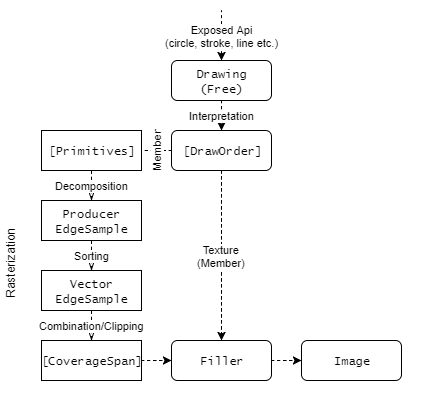
\includegraphics[width=.4\linewidth]{../rasterific-pipeline}
  \caption{Approximation of the Rasterific pipeline.}
  \label{fig:rasterific-pipeline}
\end{figure}

Figure \ref{fig:rasterific-pipeline} shows our basic understanding of the general pipeline in Rasterific. The user of the library defines a bunch of vector shapes by calling the
API which are represented internally as a series of commands in a free monad. When this is interpreted, a list of \texttt{DrawOrder} objects are generated which contain lists
of primitives (Bezier curves - linear, quadratic, and cubic) which are the pumped through a rasterization pipeline (the left wing in Figure \ref{fig:rasterific-pipeline}). The rasterization
pipeline decomposes the primitives into raster lines, sorts them, and finally combines them. Finally, a filling strategy and some texture is applied and we have an image.

Based on a discussion in Rasterifics Issue Tracker\footnote{\url{https://github.com/Twinside/Rasterific/issues/32}}, we have focused mainly on the full rasterization pipeline of
primitives, this includes the following:
\begin{enumerate}
\item the decomposition of primitives into \texttt{EdgeSample}s, a very fine-grained task with potential for constant span;
\item the sorting of \texttt{EdgeSample}s, a known problem with somewhat limited potential for parallism; and,
\item the combination of \texttt{EdgeSample}s into \texttt{CoverageSpan}s, a somewhat more complicated and course grained task with the highest potential for speedup at face value.
\end{enumerate}

It's worth noting that the Gezira library is parallel to some degree. It may be fruitful to base any parallelization efforts in Rasterific on how it is achieved in Gezira. However,
since Gezira is written in Nile and compiled into C with a heavy runtime which we would need to understand to understand when the rasterizer is multithreaded, we chosen to instead
 base our work on the comments of Rasterific's author.
%Måske noget om benchmarks?
\subsection{Parallel Haskell}
For this project, we have spent most of our time working with the Par Monad -- besides with sorting where we end up making use of the primitives in \texttt{Control.Parallel}.
 This is mainly based on ease of use. We could as well have chosen to work with Strategies, and it may
have been preferable considering the fine granularity of some of our tasks, but we feel more comfortable working with the more simple API from \texttt{Monad.Par}.
However, to make use of some of the more powerful analysis tools in ThreadScope, we make use of the spark scheduler for the Par Monad
\footnote{\url{https://hackage.haskell.org/package/monad-par-0.3.4.8/docs/Control-Monad-Par-Scheds-Sparks.html}}.

The main consequence of this choice is that the tools from the Par Monad package are hyperstrict, so we are forced to force a lot of lazy computations to enable parallelism -- pun not intended.


%Focus on Par monad (forced evaluation as opposed to lazy). Haven't needed concurrent primitives because most of the code lends itself well to parallel primitives (with the possible exception of sorting). Also it was easiest to use ...


\section{Experiments}\label{experiments}

Approach to find possibilities for parallelization: reading the salient parts of the source code and identifying them manually. We have also followed the pointers from the Rasterific author in \url{https://github.com/Twinside/Rasterific/issues/32#issuecomment-338327066}

Some kind of revised graph from the one in Section \ref{background}, with the specific functions we have worked on annotated + clearly describing which granularity they operate at. v importante

\subsection{Benchmarks}
We will make references to some benchmarks further down. This is a short recap of which benchmarks exist in Rasterific and which ones we have added.
\begin{itemize}
\item \textbf{Snowflake:} Draws a series of transparent snowflakes on a background. See Figure \ref{fig:snowflakes}. Was added to the Rasterific project
   shortly before we started our project.
\item ??
\item \textbf{Lines:} Draws a large number of randomly colored lines on a background. See Figure \ref{fig:lines-benchmark}.
  We have added this to benchmark line primitive decomposition.
\end{itemize}
\begin{figure}[h!]
  \centering
  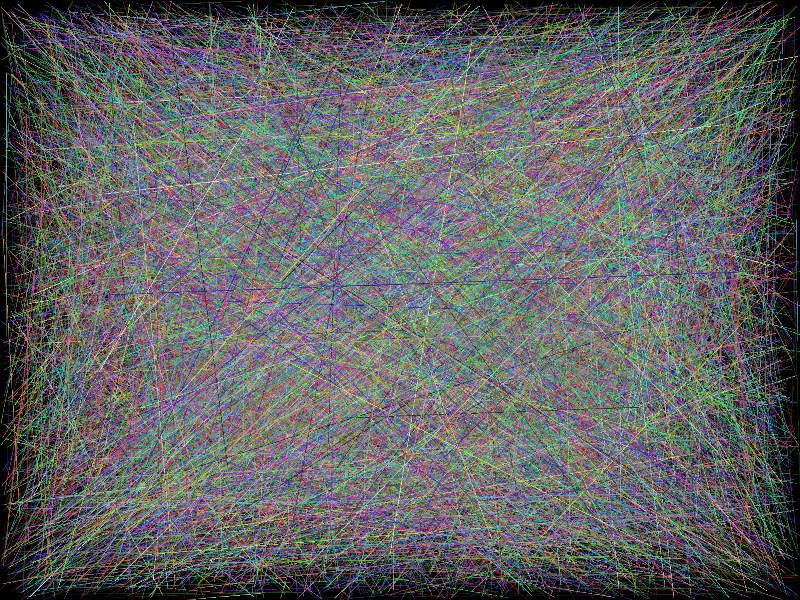
\includegraphics[width=.4\linewidth]{../lines}
  \caption{The output of the \texttt{lines} benchmark.}
  \label{fig:lines-benchmark}
\end{figure}

\subsection{Primitives}
Before rasterization, Rasterific works with three different primitive shapes:
lines, quadratic bezier curves, and cubic bezier curves. Each of these are decomposed
to an internal type representing raster lines:
\begin{lstlisting}[caption={\texttt{EdgeSample} type -- represents a raster line.}]
data EdgeSample = EdgeSample
  { _sampleX     :: {-# UNPACK #-} !Float -- ^ Horizontal position
  , _sampleY     :: {-# UNPACK #-} !Float -- ^ Vertical position
  , _sampleAlpha :: {-# UNPACK #-} !Float -- ^ Alpha
  , _sampleH     :: {-# UNPACK #-} !Float -- ^ Height
  }
\end{lstlisting}
This decomposition follows a divide-and-conquer strategy. For example, decomposing a line
involves repeatedly chopping the line in half until both endpoints are in the same pixel.

This pattern seems ripe for parallelisation, however there are a couple of shortfalls:
\begin{itemize}
\item The size of the canvas severely restricts the length of a primitive -- there is no reason to ever
   have a million pixel line.
 \item The decomposition functions returns the following lazy data structure:
   \begin{lstlisting}
     type Producer a = [a] -> [a]\end{lstlisting}
   presumably to save the cost of generating a long list of lists just to concatenate them in the end
    when the \texttt{EdgeSamples} are sorted.
  \end{itemize}
  Nevertheless, we have experimented with parallelizing the decomposition of primitives.

\subsubsection{Lines}
The \texttt{Graphics.Rasterific.Line} module has the \texttt{decomposeLine} function with type
signature:
\begin{lstlisting}
decomposeLine :: Line -> Producer EdgeSample\end{lstlisting}
The basic work this function does, is decompose a \texttt{Line} primitive into a list of
\texttt{EdgeSample}. As stated above, it does so by divide-and-conquer.

We implemented a case in the internal helper function which sparks a computation for each half of the list.
We experimented a bit with how to chunk the parallelism, and ended up with an option which initially splits
 work and then runs sequentially until depth $n$. This can be seen in Figure \ref{lst:linepar} for $n=10$.
\begin{lstlisting}[caption={Naively splitting work in two parts every 10 levels of the recursion tree.}, label={lst:linepar}]
    go !ax !ay !bx !by n cont
    | n == 0  = runPar $ do
        a' <- spawnP $ go ax ay mx my 10 []
        b' <- spawnP $ go mx my bx by 10 []
        b <- get b'
        a <- get a'
        return $ a ++ b ++ cont
\end{lstlisting}
This approach proves to not generate enough work for each thread. This is even when only a single split
is performed ($n$ is set very large). Figure \ref{fig:line-thread} shows ThreadScope out put for only splitting the
work a single time (per line) on two cores. Even with this course distribution of work
26731 of 34000 sparks end up being garbage collected, and we only manage approximately utilize 25\% of two available
 cores.

Additionally, running the parallel code with a single core (\texttt{-N1}) gives better performance than with
two.
\begin{figure}[h!]
  \centering
  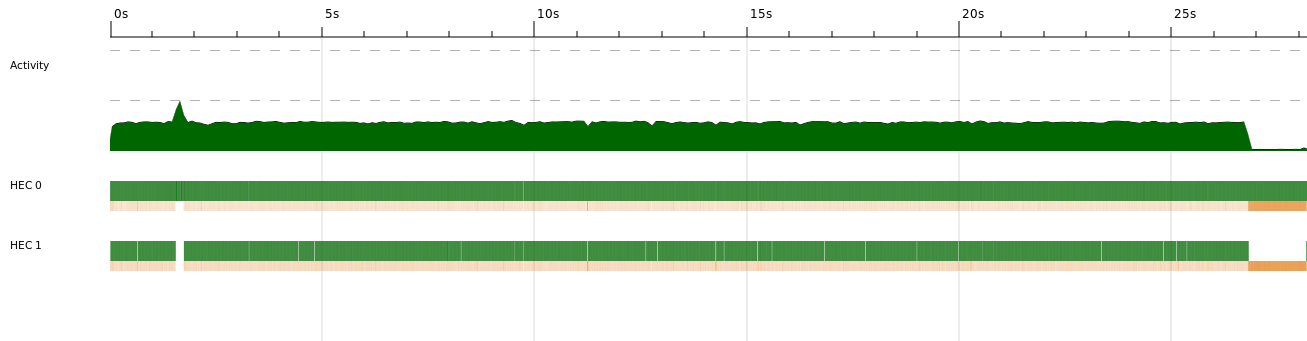
\includegraphics[width=0.85\linewidth]{../threadscope/lines/single-split}
  \caption{ThreadScope output for parallelising line decomposition. Shows the output for the
    \texttt{lines} benchmark.}
  \label{fig:line-thread}
\end{figure}

Inspecting the spark times (Figure \ref{fig:line-thread-sparks}) in ThreadScope confirms that line
decomposition does not produce work enough to justify the hassle --
probably not even to offset any cache locality reduction from working 
on multiple cores. Most of the converted sparks are completed instantaniously.

\begin{figure}[h!]
  \centering
  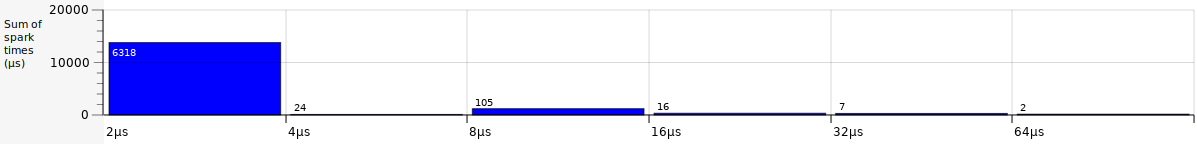
\includegraphics[width=0.85\linewidth]{../threadscope/lines/single-split-spark-times}
  \caption{ThreadScope spark times for Figure \ref{fig:line-thread}}
  \label{fig:line-thread-sparks}
\end{figure}

To investigate further, we wrote a small program that runs \texttt{decomposeLine} on a single, \textit{unrealisically} large line where
 we fork at every 10th recursive call. Figures \ref{fig:single-line-thread} and \ref{fig:single-line-thread-sparks} show the results. Again we have
 weak utilisation and small spark workloads. Given that this is probably the base case for parallisation of decomposing the line primitive there
  probably isn't must hope for any speedup here.

\begin{figure}[h!]
  \centering
  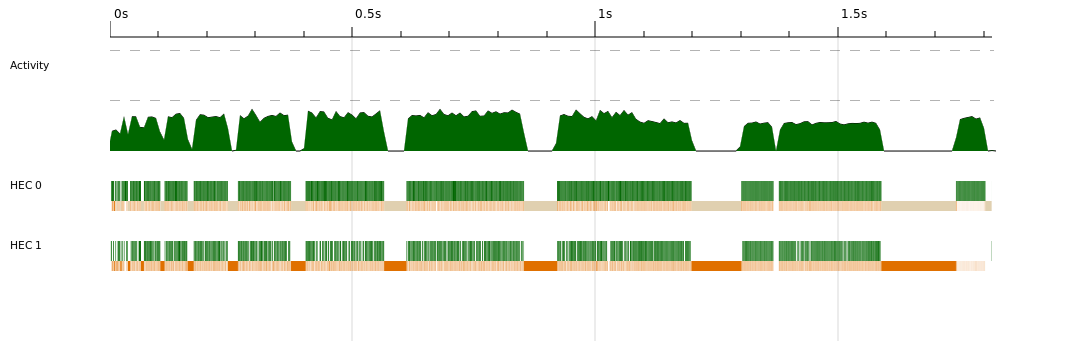
\includegraphics[width=0.85\linewidth]{../threadscope/lines/single-line-every-10}
  \caption{ThreadScope output for running line decomposition on a single line with length
    100000.}
  \label{fig:single-line-thread}
\end{figure}

\begin{figure}[h!]
  \centering
  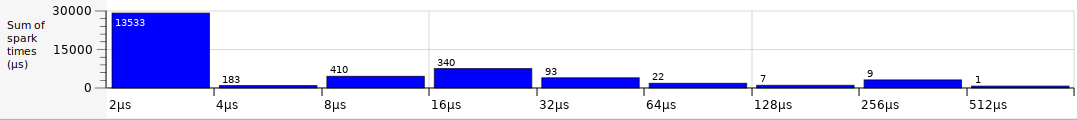
\includegraphics[width=0.85\linewidth]{../threadscope/lines/single-line-every-10-spark-times}
  \caption{ThreadScope output for running line decomposition on a single line with length
    100000.}
  \label{fig:single-line-thread-sparks}
\end{figure}

\subsection{Sorting Edge Samples}

After the Primitives have been decomposed into \texttt{EdgeSamples}, they are sorted by their y and then x coordinates (in that order).
This is done using the \texttt{vector-algorithms} package, such that the vector of \texttt{EdgeSamples} is sorted in place as a mutable vector
 using an implementation of introsort.
\begin{lstlisting}[caption={Sorting the edge samples.}]
sortEdgeSamples :: [EdgeSample] -> V.Vector EdgeSample
sortEdgeSamples samples = runST $ do
  -- Resist the urge to make this a storable vector,
  -- it is actually a pessimisation.
  mutableVector <- V.unsafeThaw $ V.fromList samples
  VS.sortBy xyCompare mutableVector
  V.unsafeFreeze mutableVector
\end{lstlisting}

Since sparking imperative code is not something you can do by default, and we want spark stats for
analysis, we can make use of a little hack (see Listing \ref{lst:parst}) which creates a sparkable
 thunk out of an ST computation found in an online discussion\footnote{\label{note1}\url{https://unlines.wordpress.com/2010/04/21/sparking-imperatives/}}\footnote{}.
\begin{lstlisting}[label={lst:parst}, caption={\texttt{parST}}]
parST :: ST s a -> ST s a
parST m = x `par` return x
  where
    x = runST (unsafeIOToST noDuplicate >> unsafeCoerce m)
\end{lstlisting}
Obviously, competing with optimized sequential code from the \texttt{vector-algorithms} package is a
 bit is a long shot, but for the sake of experiment we wrote a sorting function (based on an example from where we got the \texttt{parST} function),
 it is a parallel, in-place quicksort (Listing \ref{lst:parsort}) with a depth and size threshold for deciding when to bail out to the aforementioned intro sort.

 Figure \ref{fig:sorting-thread} shows ThreadScope output for a isolated test of the sorting function.
 It shows some good pretty alright utilisation of the two cores.

 \begin{figure}[h!]
  \centering
  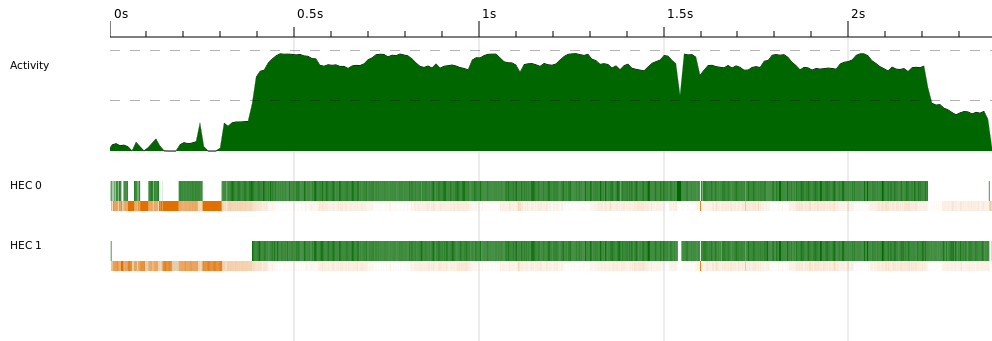
\includegraphics[width=0.85\linewidth]{../threadscope/sorting/sorting-final}
  \caption{ThreadScope output for sorting 1.000.000 \texttt{EdgeSample}s.}
  \label{fig:sorting-thread}
\end{figure}

Figure \ref{fig:sorting-thread-zoomed}, shows a zoomed in view of the middle segment of Figure \ref{fig:sorting-thread}.
This gives us the impression, once again, that we have pretty good utilisation.

 \begin{figure}[h!]
  \centering
  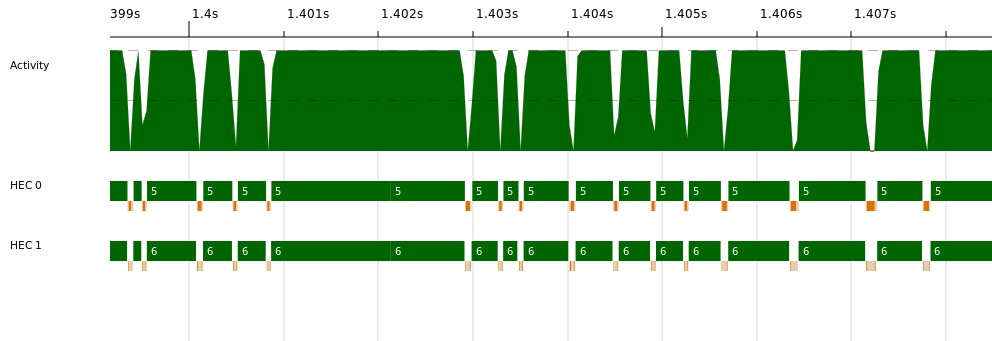
\includegraphics[width=0.85\linewidth]{../threadscope/sorting/sorting-final-zoom}
  \caption{ThreadScope output for sorting 1.000.000 \texttt{EdgeSample}s.}
  \label{fig:sorting-thread-zoomed}
\end{figure}

This is reflected in some superficial timings (using \texttt{-s}) -- taking 3.2s on one core, 2.2s on two, 1.6s on three, and 1.4s on four. The bad news is that \texttt{MV.sortBy} takes less than a second to sort the same vector.

Even worse, is that loosening up the parallisation threshold (i.e. increasing the spark production)
greatly decreases performance. Removing the thresholds alltogether results in not being able to get
 through the 1.000.000 length vector at all.
 \begin{figure}[h!]
  \centering
  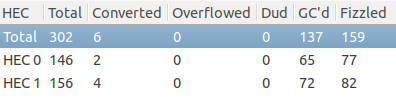
\includegraphics[width=0.6\linewidth]{../threadscope/sorting/sorting-final-sparks}
  \caption{ThreadScope spark output for sorting 1.000.000 \texttt{EdgeSample}s.}
  \label{fig:sorting-thread-sparks}
\end{figure}

Another symptom of this may be the incredibly low spark conversion rate the sorting function has.
Figure \ref{fig:sorting-thread-sparks} shows the spark conversion rate from the run shown in
Figure \ref{fig:sorting-thread}. Only 6 out of 300 sparks are converted, and 159 end up fizzling.


If we remove the threshold and decrease the vector size to 100k, we get the conversion rate in
Figure \ref{fig:sorting-thread-100k-sparks}. We only convert 5 sparks and generate \textit{two hundred thousand}. This should only be possible if we somehow had generated
a completely unbalanced comparison tree. This implies a performance bug (either in the sorting function
 itself or the \texttt{parST} hack), but we have been unable to locate it.
 \begin{figure}[h!]
  \centering
  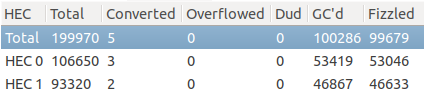
\includegraphics[width=0.6\linewidth]{../threadscope/sorting/sorting-100k-sparks}
  \caption{ThreadScope spark output for sorting 100.000 \texttt{EdgeSample}s!}
  \label{fig:sorting-thread-100k-sparks}
\end{figure}

Either way, while we weren't able to generate a method able to sort the \texttt{EdgeSample}s faster
than the sequential intro-sort, we have at least show that there is some potential for it. This
 could reached by parallising the \texttt{vector-algorithms} package.
\subsection{Combining Edge Samples}

\subsection{Multiple Decomposition Calls}

\subsection{Multiple FillOrder Calls}

\section{Discussion}\label{discussion}

Discussion of results: why are the results (good/)bad in our specific implementations? (Overhead from parallel execution, garbage collection, especially in the non-parallel parts of the code.)
Are the benchmarks good indicators for performance gained by parallelism (...probably)? Should we have used another parallelization technique (i.e. not Par monad)?

% Perhaps use this link somewher https://www.reddit.com/r/haskell/comments/747zx1/parallel_computation_in_st/
Broader discussion: what is the actual scope for parallelisation in rasterific? This is kind of an analysis we could have done before starting, but the experimental approach has its own strengths.

Add some evidence for what the scope of parallelising the specific stuff from Section \label{experiments} -- e.g. traced threadscope graphs, debug traces showing actual numbers of draworders, primitives, and edgesamples generated by our benchmarks, etc. All in all, it's very nested.

\section{Further Work}\label{furtherwork}
The work we have done for this report has been somewhat superficial constrained by the existing flow and data structures in Rasterific.
 It would be interesting to see what could be done if these constraints were up for change. Some of the following ideas could be interesting for future work.
\begin{itemize}
\item Shift Rasterific from relying on laziness, and try to unify which data strucures are used throughout the library to make it more easy to construct
  broad parallel solutions. Perhaps take a look at the Repa package.
\item Try to flatten the calls into the inner rasterization pipeline. This could perhaps enable more course grained parallelism which could be more readily exploited.
  This may require changes to the public API, but may be worth it.
\end{itemize}
%Streamlining data structures: especially in rasterize, there is a lot of conversion between data structures, as well as reliance on laziness, which is sort of terrible for the strictly evaluated parallelism.
%Perhaps bigger refactoring needed for maximum parallel gains, e.g. flattening the nested parallelism.

\section{Conclusion}
=======
\clearpage
\appendix

\section{Code}
\begin{lstlisting}[label={lst:parsort}, caption={Parallel Sorting}]
parSort :: (Show e, MV.MVector v e, Ord e) => v s e -> ST s ()
parSort a = go a $ ceiling $ log fl
  where
    fl = fromIntegral $ MV.length a
    go a d
      | n < 2 = return ()
      | d < 1 || n < 1000 = VS.sort a -- Don't bother sparking for smaller Vs
      | otherwise = do
          MV.unsafeSwap a 0 mid -- Pivot index > 0
          p <- MV.unsafeRead a 0 -- Get pivot
          let rest = MV.unsafeSlice 1 (n-1) a -- Keep pivot in place
          m' <- MV.unstablePartition (<p) rest -- Partition rest of array
          MV.unsafeSwap a 0 m' -- Swap pivot back into place m' is the first index of the second partition of rest but the last of a
          let a1 = MV.unsafeSlice 0 m' a -- {abcd}p   first slice cannot be empty; second can
          let a2 = MV.unsafeSlice (min (m'+1) n) (n-(min (m'+1) n)) a -- abcdp{efgh}
          v <- parST $ go a1 (d-1)
          v2 <- parST $ go a2 (d-1)
          v `seq` v2 `seq` return ()
            where
              n = MV.length a
              mid = n `div` 2
\end{lstlisting}%$


\begin{lstlisting}[label={lst:sorting}]
main :: IO ()
main = do
  let xs = [x | x <- [1..]] :: [Int]
      ys = [y*2 | y <- [6..]] :: [Int]
      list = take 100 [x `mod` 11 | x <- xs]
      edgesamples = [EdgeSample { _sampleX = fromIntegral  (x `mod` 10),
                                  _sampleY = fromIntegral (y `mod` 30),
                                  _sampleAlpha = (1.5::Float),
                                  _sampleH = (2.1 :: Float)
                                }
                    | x <- xs,
                      y <- ys]
      pa = take 1000000 edgesamples
  start <- getCPUTime
  let sortedPar = sortEdgeSamples pa
  end <- sortedPar `seq` getCPUTime
  let time = (fromIntegral (end - start)) / (10^12)
  printf "Time: %0.9f sec\n" (time :: Double)
\end{lstlisting}

\begin{lstlisting}[caption={Decomposing a very long single line.}, label={lst:singleline}]
import Internal (
  decomposeLine
  ,Line
  )
import Graphics.Rasterific
import Control.DeepSeq
import Debug.Trace

main :: IO ()
main = do
  let l = Line (V2 0 0) (V2 1000000 1000000)
      x = (decomposeLine l) []
  putStrLn $ deepseq x "done"
\end{lstlisting}
\end{document}
